\documentclass{article}
\usepackage{graphicx}
\usepackage[margin=1in]{geometry} 
\usepackage{float}
\usepackage{xcolor}
\usepackage{hyperref}
\usepackage{float}
 
\begin{document}

\title{Project 4 - Facebook API and Simulator \\ COP5615, Fall 2015}
 
\author{Grant Hernandez and Chelsea Metcalf}
 
\maketitle % this produces the title block
 
\section*{Code Structure}
Client/Server
\begin{figure}[H]
  \centering
  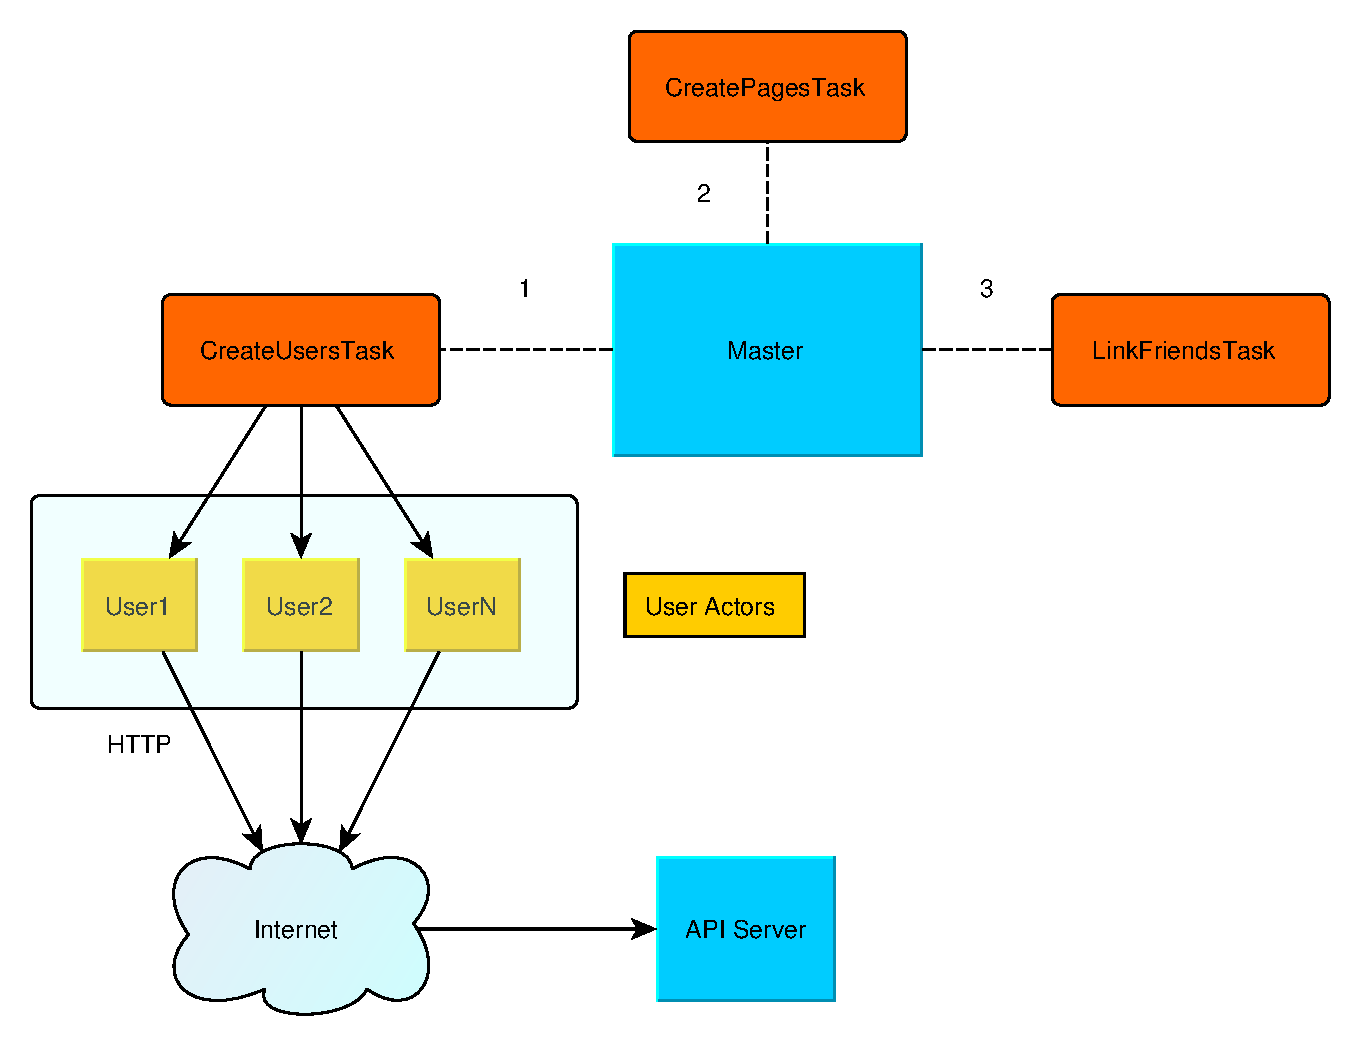
\includegraphics[scale=0.5]{diagrams/client-structure.pdf}
  \label{cli-struct}
  \caption{Client structure}
\end{figure}

\begin{figure}[H]
  \centering
  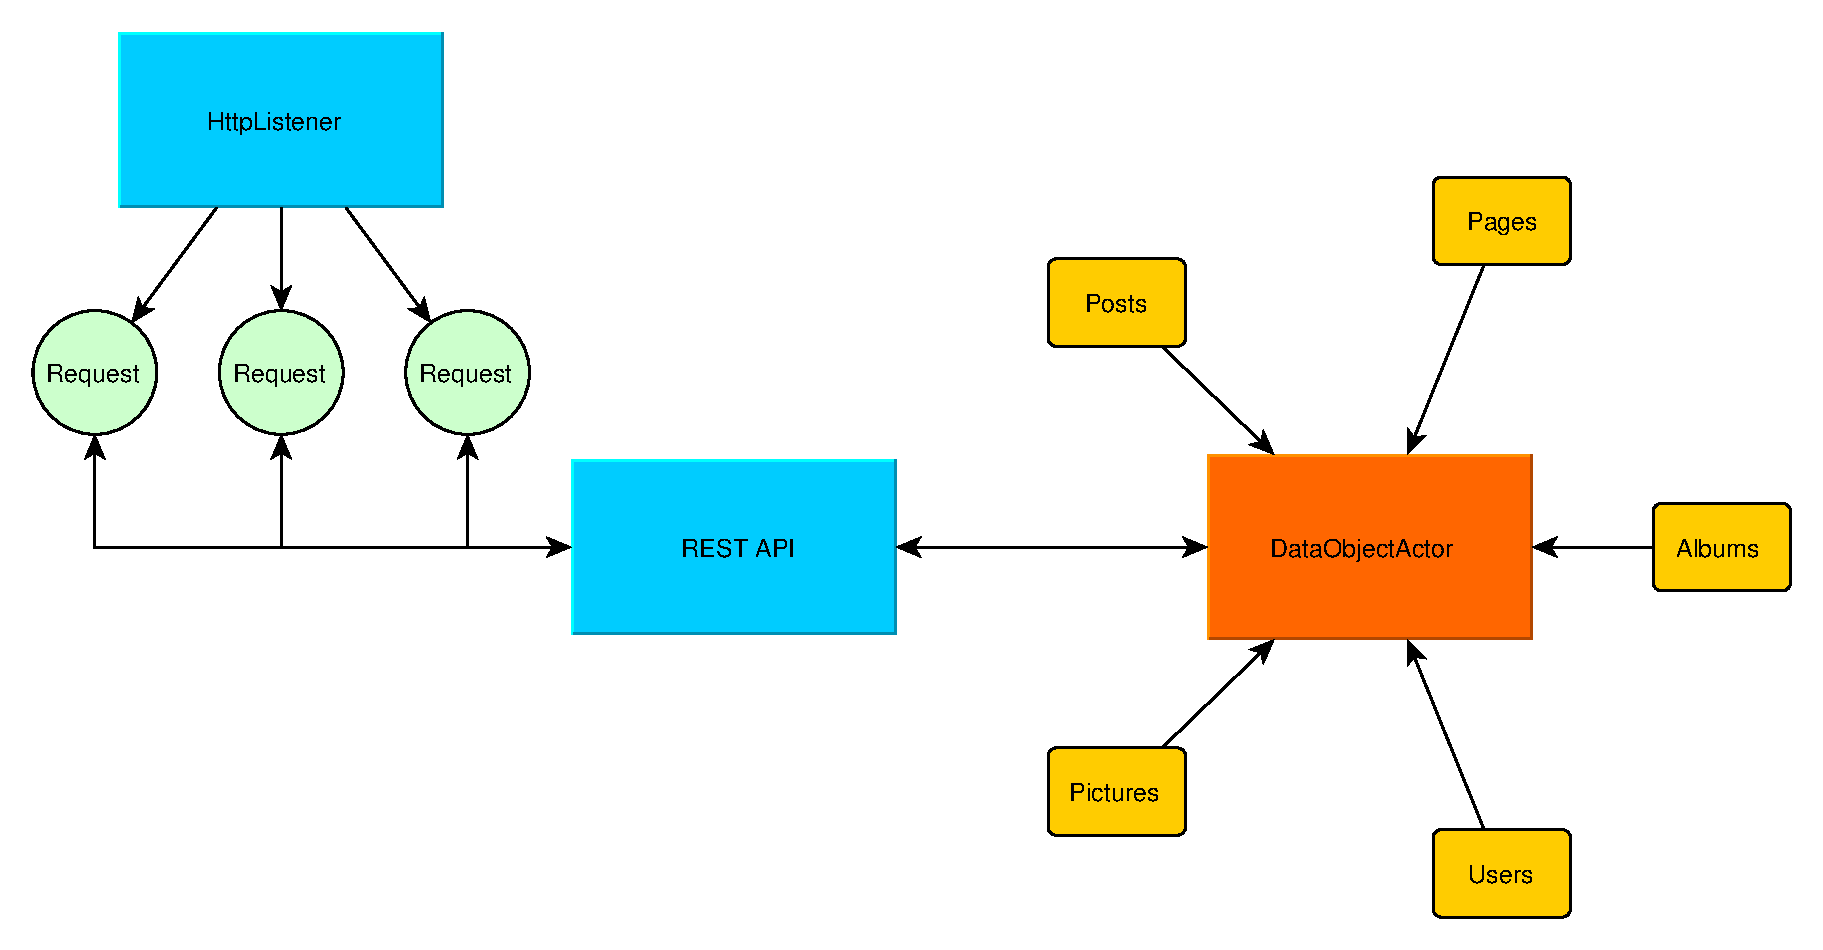
\includegraphics[scale=0.5]{diagrams/server-structure.pdf}
  \label{svr-struct}
  \caption{Server structure}
\end{figure}

\subsection*{Client Simulator}

\subsection*{API Server}
The API server utilizes Spray to build a REST API. In each unique REST route either an entity is deserialized using Spray-JSON or parameters are extracted from the route URI. Once the inputs are extracted, they are passed by message, along with the \texttt{RequestContext} to a data manager Actor. This actor serializes requests to Facebook data objects and implements all of the business logic for the site. This includes creating users, pages, posts, albums, and pictures. It also allows these items to be looked up by ID and retrieved. Additionally, auxiliary functions such as adding friends are implemented here due to the easy data object access.

One limitation of this approach is that all of the data objects are stored in one Actor instance. This makes programming easy, but since actors are single threaded and can only process one message at a time, this becomes a limitation. A solution to this would be to have a more generic way of storing data such that any Actor could manage a chunk of user data. Then the API frontend would have to message a router to figure out which Actor was responsible for the required objects. This would increase the parallelism of the API server.

\section*{User Studies}
We generated our users based on these user studies. They are a combination of actual Facebook studies and studies on the general population.
\subsection*{Age}
\begin{table}[H]
\centering
\begin{tabular}{|p{2cm}||p{2cm}|} 
 \hline
 Age & Percentage \\ [0.5ex] 
 \hline\hline
 13 - 17 & 0 percent \\
 \hline
 18 - 24 & 15 percent \\
 \hline
 25 - 34 & 29 percent \\
 \hline
 35 - 44 & 24 percent \\ [1ex] 
 \hline
\end{tabular}
\caption{Age Study \cite{sproutsocialwebsite}}
\label{table:1}
\end{table}

\subsection*{Relationship Status}
\begin{table}[H]
\centering
\begin{tabular}{|p{3cm}||p{3cm}|} 
 \hline
 Relationship Status & Percentage \\ [0.5ex] 
 \hline\hline
 Single & 37 percent \\
 \hline
 Married & 31 percent \\
 \hline
 In a Relationship & 24 percent \\
 \hline
 Engaged & 3 percent \\
 \hline
 It's Complicated & 3 percent \\ [1ex] 
 \hline
\end{tabular}
\caption{Relationship Status Study \cite{relstatuswebsite}}
\label{table:2}
\end{table}

\subsection*{Political Affiliation}
\begin{table}[H]
\centering
\begin{tabular}{|p{3cm}||p{3cm}|} 
 \hline
 Party Affiliation & Percentage \\ [0.5ex] 
 \hline\hline
 Republicans & 25 percent \\
 \hline
 Democrats & 29 percent \\
 \hline
 Independents & 41 percent \\ [1ex] 
 \hline
\end{tabular}
\caption{Political Affiliation Study \cite{polstatuswebsite}}
\label{table:3}
\end{table}

\subsection*{Interested In}
\begin{table}[H]
\centering
\begin{tabular}{|p{3cm}||p{3cm}|} 
 \hline
 Interested In & Percentage \\ [0.5ex] 
 \hline\hline
 Straight & 96.6 percent \\
 \hline
 Gay/Lesbian & 2.4 percent \\
 \hline
 Bisexual & 0.7 percent \\ [1ex] 
 \hline
\end{tabular}
\caption{Political Affiliation Study \cite{interestedinwebsite}}
\label{table:4}
\end{table}

\subsection*{Facebook Activity}
\begin{figure}[H]
  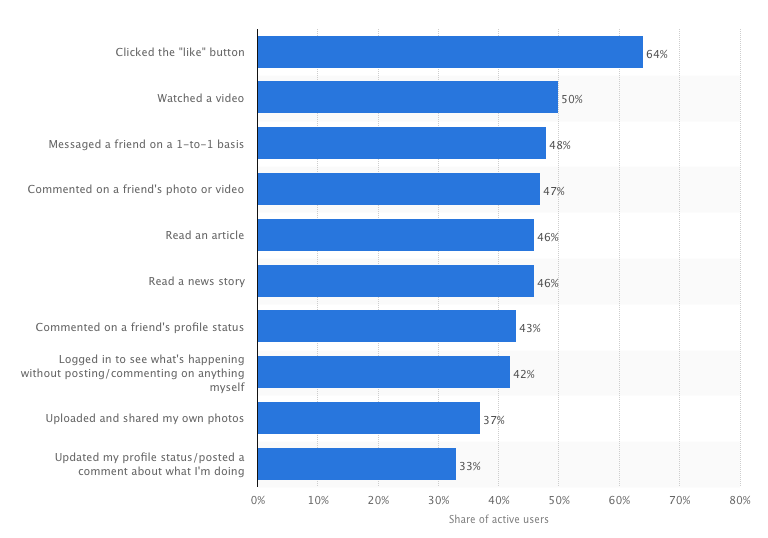
\includegraphics[width=\linewidth]{fbact.png}
  \caption{Share of Active Users. \cite{fbactwebsite} We did not have time to implement Facebook activity according to user statistics, but we found some interesting studies on active users.}
  \label{fig:fbact}
\end{figure}

\section*{Testing}
Tests

%%%%%%%%%%%%%%%%%%%%%%%%%%%%%%%%%%%%%%
% Begin References
%%%%%%%%%%%%%%%%%%%%%%%%%%%%%%%%%%%%%%
\begin{thebibliography}{99}

\bibitem{sproutsocialwebsite} 
Social Media Demographics to Inform a Better Segmentation Strategy,
\\\texttt{http://sproutsocial.com/insights/new-social-media-demographics/}

\bibitem{relstatuswebsite} 
Facebook Relationship Status Statistics,
\\\texttt{http://www.statisticbrain.com/facebook-relationship-status-statistics/}

\bibitem{polstatuswebsite} 
Party Affiliation,
\\\texttt{http://www.gallup.com/poll/15370/party-affiliation.aspx}

\bibitem{interestedinwebsite} 
What percentage of the U.S. population is gay, lesbian, or bisexual?,
\\\texttt{https://www.washingtonpost.com/news/volokh-conspiracy/wp/2014/07/15/
what-percentage-of-the-u-s-population-is-gay-lesbian-or-bisexual/}

\bibitem{girlnameswebsite} 
Most Popular Girl Names in 2014,
\\\texttt{http://www.babycenter.com/popular-baby-girl-names-2014}

\bibitem{boynameswebsite} 
Most Popular Boy Names in 2014,
\\\texttt{http://www.babycenter.com/popular-baby-boy-names-2014}

\bibitem{lastnameswebsite} 
Most Popular Last Names,
\\\texttt{https://en.wikipedia.org/wiki/ListofmostcommonsurnamesinNorthAmerica}

\bibitem{fbactwebsite} 
Most popular activities of Facebook users worldwide as of 3rd quarter 2015
\\\texttt{http://www.statista.com/statistics/420714/top-facebook-activities-worldwide/}

\bibitem{randomgeneratorcontent} 
Watchout4Snakes,
\\\texttt{http://watchout4snakes.com/wo4snakes/Random/RandomPhrase}

\end{thebibliography}

\end{document}

\end{document}
